% Provenance (never printed): see sources/outline_sources.md (Year 3: the heat
% equation, half-space and plate cooling models, heat flow against age,
% continental geotherms, thermal subsidence). Brief: sources/book5/BRIEFS.md,
% ch. 5. Curves from figdata/bachelor-3/plate_cooling.py (models; Seton et al.
% 2020 age grid and ETOPO1, read only) and continental_geotherm.py.
% Exercise and problem values in the Book 5 scratch calculator calc/ch05.py.
\chapter{Modelos térmicos da litosfera}\label{ch:b3:lithosphere-thermal-models}

Afastando-se de uma dorsal meso-oceânica, o fundo do mar se aprofunda: cerca de
\qty{2.5}{km} no eixo, mais de \qty{5}{km} sob o assoalho oceânico
mais antigo. Nada foi acrescentado à placa nem retirado dela; ela apenas
esfriou, contraiu-se e afundou. O assoalho oceânico é um termômetro da placa
sob ela, e uma sonda de fluxo de calor cravada em seus sedimentos registra o mesmo
resfriamento visto de cima. Este capítulo resolve o resfriamento de uma placa de duas maneiras, como
um semiespaço e como uma placa de espessura finita, compara ambas com a profundidade
real do assoalho oceânico e seu fluxo de calor, e depois passa aos continentes,
cujo calor provém em parte da própria crosta.
% ledger: ps77:depth-age

\begin{recall}
A equação de difusão do calor, $\partial T/\partial t = \kappa\nabla^2T$,
com a condutividade térmica $k$ e a difusividade térmica $\kappa =
k/(\rho c)$, é dos livros de física; as séries de Fourier e a função erro
$\operatorname{erf}x = (2/\sqrt\pi)\int_0^xe^{-u^2}\,\mathrm du$ estão nos
volumes universitários dos livros de matemática. O fluxo de calor, a produção radiogênica de calor
de calor, a geoterma, a escala de tempo condutivo $L^2/\kappa$, a camada limite térmica
e a litosfera térmica foram definidos no volume do primeiro ano, no
seu capítulo sobre o balanço de calor da Terra; a isostasia, no seu capítulo sobre isostasia
e anomalias gravimétricas; a lei profundidade--idade $d = d_r + C\sqrt t$ foi demonstrada em
seu capítulo sobre riftes, dorsais e margens passivas, admitindo o perfil de temperatura
que este capítulo deduz. O modelo de estiramento de bacias, a subsidência pós-rifte
e a constante de tempo térmica estão no volume do segundo ano, no seu
capítulo sobre bacias sedimentares.
\end{recall}

\section{Condução, advecção e sua razão}

O calor na litosfera se move de duas maneiras: difunde-se no sentido do gradiente
de temperatura e é transportado pela rocha em movimento, como a placa que se afasta de uma dorsal, uma
montanha erodida que se eleva, um magma que ascende. Qual dos dois predomina depende de um único
número.

\begin{definition}[Número de Péclet térmico]\label{def:b3:lithosphere-thermal-models:peclet}
Para uma rocha que se move com velocidade $u$ ao longo de um comprimento $L$, o \emph{número de Péclet
térmico}\index{número de Péclet térmico} é
\[
  \mathrm{Pe} = \frac{uL}{\kappa},
\]
a razão entre o tempo condutivo $L^2/\kappa$ e o tempo advectivo $L/u$.
A advecção domina onde $\mathrm{Pe} \gg 1$, e a condução onde
$\mathrm{Pe} \ll 1$.
\end{definition}

Uma placa que se afasta de uma dorsal a \qty{25}{mm/yr} apresenta, ao longo de uma distância de
\qty{95}{km}, $\mathrm{Pe} \approx 94$ com $\kappa = \qty{0.8e-6}{m^2.s^{-1}}$:
o calor é transportado lateralmente pela placa muito mais depressa do que se difunde lateralmente.
Cada coluna vertical da placa, portanto, esfria como se estivesse isolada, por condução
vertical até o assoalho oceânico frio, sendo sua idade $t$ o tempo decorrido desde que
deixou o eixo. Isso transforma um problema bidimensional em um problema de profundidade e
tempo.

\section{O semiespaço em resfriamento}

\begin{definition}[Modelo de resfriamento do semiespaço]\label{def:b3:lithosphere-thermal-models:half-space}
O \emph{modelo de resfriamento do semiespaço}\index{modelo de resfriamento do semiespaço} da
litosfera oceânica toma cada coluna como um semiespaço $z \ge 0$ de difusividade uniforme,
à temperatura uniforme $T_m$ do manto quando ela deixa o eixo da dorsal,
cuja superfície é mantida, desde então, na temperatura $T_0$ do
assoalho oceânico, sem produção de calor e sem base.
\end{definition}

\begin{theorem}[Geoterma em função erro]\label{thm:b3:lithosphere-thermal-models:erf}
No \omterm{def:b3:lithosphere-thermal-models:half-space}{modelo de resfriamento do semiespaço}, a temperatura na profundidade $z$ abaixo do
assoalho oceânico de idade $t$ é
\[
  T(z, t) = T_0 + (T_m - T_0)\operatorname{erf}\frac{z}{2\sqrt{\kappa t}} .
\]
Essa é a \emph{geoterma em função erro}\index{geoterma em função erro}.
\end{theorem}

\begin{proof}
Seja $\theta = (T - T_0)/(T_m - T_0)$; ele resolve $\partial\theta/\partial t =
\kappa\,\partial^2\theta/\partial z^2$ com $\theta(z, 0) = 1$ para $z > 0$ e
$\theta(0, t) = 0$ para $t > 0$. O problema não tem escala de comprimento própria:
se $\theta(z, t)$ é uma solução, também o é $\theta(\lambda z, \lambda^2t)$ para todo
$\lambda > 0$, com os mesmos valores inicial e de contorno; sendo a solução
única, $\theta$ depende de $z$ e $t$ somente por meio de $\eta = z/(2\sqrt{\kappa
t})$. Escrevendo $\theta = f(\eta)$, com $\partial\eta/\partial t = -\eta/(2t)$ e
$\partial\eta/\partial z = 1/(2\sqrt{\kappa t})$,
\[
  -\frac{\eta}{2t}f'(\eta) = \kappa\,\frac{f''(\eta)}{4\kappa t},
  \qquad\text{logo}\qquad f'' + 2\eta f' = 0 .
\]
Logo $f' = Ae^{-\eta^2}$ e $f = A\int_0^\eta e^{-u^2}\,\mathrm du + B$. A
condição na superfície, em $\eta = 0$, dá $B = 0$; a condição inicial, que
vale em toda profundidade quando $t \to 0$, isto é, quando $\eta \to \infty$, dá
$A\sqrt\pi/2 = 1$. Assim, $f = \operatorname{erf}\eta$.
\end{proof}

A temperatura em uma dada profundidade depende apenas de $z/\sqrt t$: uma isoterma afunda
proporcionalmente à raiz quadrada da idade, e a camada resfriada a \qty{40}{Myr} é duas
vezes mais espessa do que a \qty{10}{Myr}. O fluxo de calor na superfície segue por derivação.

\begin{proposition}[Relação entre fluxo de calor e idade]\label{prop:b3:lithosphere-thermal-models:heat-flow}
No \omterm{def:b3:lithosphere-thermal-models:half-space}{modelo de resfriamento do semiespaço}, o fluxo de calor através do assoalho oceânico de idade $t$
é
\[
  q(t) = k\,\frac{\partial T}{\partial z}\Big|_{z=0}
  = \frac{k(T_m - T_0)}{\sqrt{\pi\kappa t}} = \frac{C_q}{\sqrt t} .
\]
\end{proposition}

\begin{proof}
$\partial\operatorname{erf}(z/2\sqrt{\kappa t})/\partial z = (2/\sqrt\pi)
e^{-z^2/4\kappa t}/(2\sqrt{\kappa t})$, que em $z = 0$ é $1/\sqrt{\pi\kappa
t}$.
\end{proof}

Com os valores do modelo de placa abaixo ($k = \qty{3.1}{W.m^{-1}.K^{-1}}$,
$T_m - T_0 = \qty{1450}{K}$, $\kappa = \qty{0.8e-6}{m^2.s^{-1}}$), $C_q =
\qty{505}{mW.m^{-2}.Myr^{1/2}}$, próximo dos valores de 430 a
\qty{510}{mW.m^{-2}.Myr^{1/2}} ajustados às medições globais feitas por diferentes
estudos; uma compilação recente prefere \num{490}. O fluxo de calor medido na
crosta oceânica jovem, no entanto, subestima grosseiramente o calor que dela sai:
a água do mar que circula pela crosta fraturada leva parte do calor embora
em fontes hidrotermais, fora do alcance das sondas. Sobre a crosta antiga, as medições
seguem $1/\sqrt t$, e as estimativas da perda de calor da Terra substituem as
medições na crosta mais jovem que \qty{66.5}{Myr} por $C_q/\sqrt t$.
% ledger: honda04:gdh1, b2dd10:half-space, dd10b5:hydrothermal

O volume do primeiro ano integrou o mesmo perfil em profundidade, por meio da isostasia, para
obter a lei profundidade--idade, $d = d_r + C\sqrt t$ com $C = 2\rho_m\alpha(T_m -
T_0)\sqrt\kappa/\bigl(\sqrt\pi(\rho_m - \rho_w)\bigr)$ (figura abaixo). Com
$\rho_m = \qty{3300}{kg.m^{-3}}$, $\rho_w = \qty{1030}{kg.m^{-3}}$ e $\alpha =
\qty{3.1e-5}{K^{-1}}$, $C = \qty{370}{m.Myr^{-1/2}}$, frente aos
\qty{350}{m.Myr^{-1/2}} ajustados aos assoalhos do Pacífico Norte e do Atlântico Norte
mais jovens que \qty{70}{Myr}.
% ledger: ps77:depth-age

\begin{omfigure}
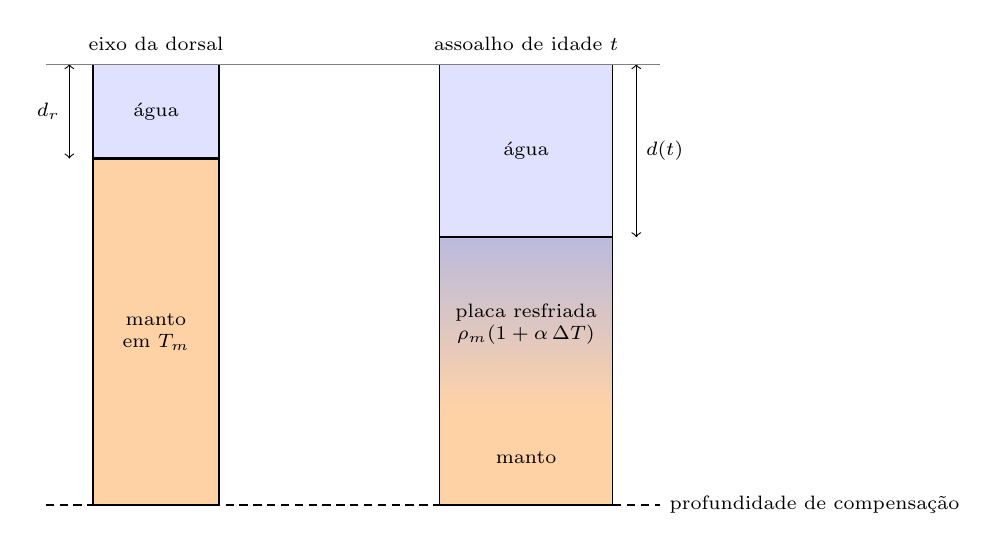
\begin{tikzpicture}[font=\small, x=1cm, y=1cm]
% schematic: two columns of equal mass above the compensation depth
\fill[blue!12] (0,0) rectangle (1.6,-1.2);
\fill[orange!35] (0,-1.2) rectangle (1.6,-5.6);
\fill[blue!12] (4.4,0) rectangle (6.6,-2.2);
\shade[top color=blue!35!gray!40, bottom color=orange!35] (4.4,-2.2) rectangle (6.6,-4.4);
\fill[orange!35] (4.4,-4.4) rectangle (6.6,-5.6);
\draw (0,0) rectangle (1.6,-5.6) (4.4,0) rectangle (6.6,-5.6);
\draw[densely dashed] (-0.6,-5.6) -- (7.2,-5.6) node[right, font=\scriptsize] {profundidade de compensação};
\draw[thick] (0,-1.2) -- (1.6,-1.2) (4.4,-2.2) -- (6.6,-2.2);
\node[font=\scriptsize] at (0.8,-0.6) {água};
\node[font=\scriptsize, align=center] at (0.8,-3.4) {manto\\em $T_m$};
\node[font=\scriptsize] at (5.5,-1.1) {água};
\node[font=\scriptsize, align=center] at (5.5,-3.3) {placa resfriada\\$\rho_m(1 + \alpha\,\Delta T)$};
\node[font=\scriptsize, align=center] at (5.5,-5.0) {manto};
\draw[<->] (-0.3,0) -- (-0.3,-1.2) node[midway, left, font=\scriptsize] {$d_r$};
\draw[<->] (6.9,0) -- (6.9,-2.2) node[midway, right, font=\scriptsize] {$d(t)$};
\node[above, font=\scriptsize] at (0.8,0.05) {eixo da dorsal};
\node[above, font=\scriptsize] at (5.5,0.05) {assoalho de idade $t$};
\draw[gray] (-0.6,0) -- (7.2,0);
\end{tikzpicture}

\par\smallskip{\small Isostasia da placa em resfriamento: a coluna sobre a dorsal
e a coluna de idade $t$ têm a mesma massa acima da profundidade de compensação. A
placa resfriada, mais densa, afunda, e a água preenche o espaço acima
dela.}\label{fig:b3:lithosphere-thermal-models:columns}
\end{omfigure}

\section{O modelo de placa}

O assoalho oceânico antigo deixa de se aprofundar: no Pacífico Norte e no Atlântico Norte a
profundidade se afasta de $\sqrt t$ entre 60 e \qty{80}{Myr}, e o fluxo de calor se
estabiliza. O semiespaço continua se resfriando para sempre; algo precisa manter a base da
placa aquecida.
% ledger: parsons:plate-model

\begin{definition}[Modelo de resfriamento de placa]\label{def:b3:lithosphere-thermal-models:plate}
O \emph{modelo de resfriamento de placa}\index{modelo de resfriamento de placa} da
litosfera oceânica considera cada coluna como uma camada $0 \le z \le L$ de difusividade
uniforme, na temperatura uniforme $T_m$ ao deixar a dorsal, cuja
superfície é mantida em $T_0$, e a base, em $T_m$ a partir de então.
\end{definition}

\begin{theorem}[Série de temperatura do modelo de placa]\label{thm:b3:lithosphere-thermal-models:plate-series}
No \omterm{def:b3:lithosphere-thermal-models:plate}{modelo de resfriamento de placa}, com $T_0 = 0$,
\[
  T(z, t) = T_m\Bigl[\frac zL + \frac2\pi\sum_{n=1}^\infty\frac1n
  \sin\frac{n\pi z}{L}\,e^{-n^2t/\tau}\Bigr],\qquad
  \tau = \frac{L^2}{\pi^2\kappa} .
\]
Esta é a \emph{série de temperatura do modelo de placa}\index{série de temperatura do modelo de placa}.
\end{theorem}

\begin{proof}
O estado estacionário, atingido quando $t \to \infty$, é o perfil linear $T_mz/L$.
O desvio $u = T - T_mz/L$ resolve a equação da difusão com $u = 0$ em
$z = 0$ e $z = L$, e parte de $u(z, 0) = T_m(1 - z/L)$. Separando as
variáveis, $u = Z(z)\Theta(t)$ resulta em $Z''/Z = \Theta'/(\kappa\Theta) = -\mu^2$;
as condições de contorno dão $Z = \sin(n\pi z/L)$, $\mu = n\pi/L$, e
$\Theta = e^{-n^2\pi^2\kappa t/L^2} = e^{-n^2t/\tau}$. Os valores iniciais fixam os
coeficientes $b_n$ da série de senos de $T_m(1 - z/L)$ em $[0, L]$:
\[
  b_n = \frac2L\int_0^LT_m\Bigl(1 - \frac zL\Bigr)\sin\frac{n\pi z}{L}\,\mathrm dz
  = \frac{2T_m}{n\pi},
\]
por integração por partes. Somando os modos obtém-se a série.
\end{proof}

Cada modo decai com seu próprio tempo, $\tau/n^2$: os harmônicos superiores, a estrutura fina
do degrau inicial, anulam-se primeiro, e após um tempo da ordem de $\tau$
resta apenas o primeiro. A mesma separação de variáveis dá o fluxo de
calor e, pelo balanço isostático da figura acima, a profundidade.

\begin{proposition}[Profundidade e fluxo de calor do modelo de placa]\label{prop:b3:lithosphere-thermal-models:plate-depth}
No \omterm{def:b3:lithosphere-thermal-models:plate}{modelo de resfriamento de placa}, com as densidades e a expansão térmica
da lei profundidade--idade,
\[
  q(t) = \frac{kT_m}{L}\Bigl[1 + 2\sum_{n=1}^\infty e^{-n^2t/\tau}\Bigr],\qquad
  d(t) = d_r + \frac{\rho_m\alpha T_mL}{2(\rho_m - \rho_w)}
  \Bigl[1 - \frac{8}{\pi^2}\sum_{n\ \text{ímpar}}\frac{e^{-n^2t/\tau}}{n^2}\Bigr].
\]
Quando $t \to \infty$, a profundidade tende a $d_r + \rho_m\alpha T_mL/\bigl(2(\rho_m -
\rho_w)\bigr)$ e o fluxo de calor a $kT_m/L$, ambos exponencialmente, com a
constante de tempo $\tau$.
\end{proposition}

\begin{proof}
Derivando a série em $z = 0$, $\partial T/\partial z = (T_m/L)[1 +
2\sum e^{-n^2t/\tau}]$. Para a profundidade, o equilíbrio isostático fornece $(\rho_m -
\rho_w)(d - d_r) = \rho_m\alpha\int_0^L(T_m - T)\,\mathrm dz$. A parte linear
contribui com $T_mL/2$; cada modo contribui com $-(2T_m/n\pi)e^{-n^2t/\tau}
\int_0^L\sin(n\pi z/L)\,\mathrm dz = -(2T_m/n\pi)(L/n\pi)(1 - \cos n\pi)
e^{-n^2t/\tau}$, que é nulo para $n$ par e $-(4T_mL/n^2\pi^2)
e^{-n^2t/\tau}$ para $n$ ímpar. Fatorando $T_mL/2$ obtém-se o colchete. Em $t = 0$
ele se anula, pois $\sum_{n\ \text{ímpar}}1/n^2 = \pi^2/8$.
\end{proof}

O modelo de placa que melhor se ajusta às profundidades e aos fluxos de calor globais tem uma placa
de \qty{95}{km} de espessura, com base a \qty{1450}{\celsius}, $\alpha =
\qty{3.1e-5}{K^{-1}}$ e $k = \qty{3.1}{W.m^{-1}.K^{-1}}$, mais fina e mais quente
que os valores anteriores de \qty{125}{km} e \qty{1350}{\celsius}. Com $\kappa =
\qty{0.8e-6}{m^2.s^{-1}}$, $\tau = \qty{36.2}{Myr}$; a profundidade se estabiliza em
$2500 + 3104 = \qty{5604}{m}$ e o fluxo de calor em \qty{47}{mW.m^{-2}}. O assoalho
jovem não permite distinguir os dois modelos: eles diferem por menos de um metro a
\qty{2}{Myr}, por \qty{100}{m} a \qty{44}{Myr}. A sismologia dá uma resposta
semelhante: as \omterm{def:b3:seismology-imaging:surface-waves}{ondas de Rayleigh} do Pacífico são melhor ajustadas por placas de
resfriamento cuja espessura assintótica está entre 85 e \qty{95}{km}.
% ledger: honda04:gdh1, ps77:depth-age, fischer:lithosphere

\begin{omfigure}
\begin{tikzpicture}
\begin{groupplot}[group style={group size=1 by 2, vertical sep=2.3cm},
  omrecord, width=0.86\linewidth, height=0.42\linewidth, xmin=0, xmax=160,
  xlabel={idade do assoalho oceânico (Myr)}]
\nextgroupplot[omdepth, ylabel={profundidade (km)}, ymin=0, ymax=130,
  title={(a) isotermas, a cada \qty{200}{\celsius}}, title style={font=\small},
  legend style={font=\scriptsize, at={(0.01,0.03)}, anchor=south west}]
% computed in figdata/bachelor-3/plate_cooling.py; ledger: honda04:gdh1
\addplot[omDef, thick] table[x=t, y=hs200] {figdata/out/bachelor-3-plate_cooling-isotherms.dat};
\addlegendentry{semiespaço}
\addplot[red!70!black, thick, densely dashed] table[x=t, y=pl200] {figdata/out/bachelor-3-plate_cooling-isotherms.dat};
\addlegendentry{placa, $L = \qty{95}{km}$}
\foreach \lev in {400,600,800,1000,1200,1400} {
  \addplot[omDef, thick, forget plot] table[x=t, y=hs\lev] {figdata/out/bachelor-3-plate_cooling-isotherms.dat};
  \addplot[red!70!black, thick, densely dashed, forget plot] table[x=t, y=pl\lev] {figdata/out/bachelor-3-plate_cooling-isotherms.dat};
}
\draw[gray] (axis cs:0,95) -- (axis cs:160,95);
\node[font=\scriptsize, anchor=north] at (axis cs:68,96) {base da placa};
\node[font=\scriptsize, fill=white, inner sep=1pt] at (axis cs:150,14) {200};
\node[font=\scriptsize, fill=white, inner sep=1pt] at (axis cs:28,38.2) {1000};
\node[font=\scriptsize, fill=white, inner sep=1pt] at (axis cs:22,70.4) {1400};
\nextgroupplot[ylabel={fluxo de calor (\unit{mW.m^{-2}})}, ymin=0, ymax=300,
  title={(b) fluxo de calor}, title style={font=\small},
  legend style={font=\scriptsize, at={(0.98,0.97)}, anchor=north east}]
\addplot[omDef, thick] table[x=t, y=hs] {figdata/out/bachelor-3-plate_cooling-heat.dat};
\addlegendentry{semiespaço}
\addplot[red!70!black, thick, densely dashed] table[x=t, y=pl] {figdata/out/bachelor-3-plate_cooling-heat.dat};
\addlegendentry{placa}
\end{groupplot}
\end{tikzpicture}

\par\smallskip{\small Os dois modelos de resfriamento com os parâmetros do texto.
(a) Profundidade das isotermas de \qty{200}{\celsius} (no topo) a
\qty{1400}{\celsius} (na base): as do semiespaço continuam a afundar como
$\sqrt t$, as da placa param quando o perfil se torna linear. (b) Fluxo de calor
na superfície: o modelo de placa se estabiliza em \qty{47}{mW.m^{-2}}, enquanto o
semiespaço cai como $1/\sqrt t$.}\label{fig:b3:lithosphere-thermal-models:isotherms}
\end{omfigure}

O assoalho oceânico real pode ser colocado no mesmo gráfico (figura abaixo). Cada célula
de um grau de latitude e longitude cuja idade é conhecida é colocada na sua idade e na sua
profundidade; a mediana de cada faixa de cinco milhões de anos cresce com a idade como
os modelos preveem nos primeiros \qty{40}{Myr}, mas o assoalho observado é mais raso
que ambos os modelos, e cada vez mais à medida que envelhece. Nada foi corrigido: o assoalho
antigo tem um manto de sedimentos mais espesso, de mais de um quilômetro no Atlântico Norte
mais antigo, que o sobrecarrega e eleva o seu topo, e o assoalho antigo teve tempo de
acumular montes submarinos, platôs vulcânicos e as elevações das plumas do manto.
Os ajustes publicados retiram primeiro a carga de sedimentos e as elevações evidentes; a
lei profundidade--idade do volume do primeiro ano, e os modelos de placa acima, provêm
de profundidades corrigidas desse modo.
% ledger: data:b5-depth-age, ps77:depth-age

\begin{omfigure}
\begin{tikzpicture}
\begin{axis}[omrecord, omdepth, width=0.86\linewidth, height=0.5\linewidth,
  xmin=0, xmax=180, ymin=2, ymax=6.5, xlabel={idade do assoalho oceânico (Myr)},
  ylabel={profundidade (km)},
  legend style={font=\scriptsize, at={(0.5,-0.24)}, anchor=north, cells={anchor=west}},
  legend columns=2]
% computed in figdata/bachelor-3/plate_cooling.py; ledger: data:b5-depth-age, honda04:gdh1
\addplot[only marks, mark=*, mark size=1.3pt, black,
  error bars/.cd, y dir=both, y explicit]
  table[x=t, y expr=\thisrow{med}/1000, y error plus expr=(\thisrow{q3}-\thisrow{med})/1000,
  y error minus expr=(\thisrow{med}-\thisrow{q1})/1000] {figdata/out/bachelor-3-plate_cooling-bins.dat};
\addlegendentry{observado, mediana e quartis}
\addplot[omDef, thick] table[x=t, y expr=\thisrow{hs}/1000] {figdata/out/bachelor-3-plate_cooling-depth.dat};
\addlegendentry{semiespaço}
\addplot[red!70!black, thick, densely dashed] table[x=t, y expr=\thisrow{pl}/1000] {figdata/out/bachelor-3-plate_cooling-depth.dat};
\addlegendentry{placa, $L = \qty{95}{km}$}
\end{axis}
\end{tikzpicture}

\par\smallskip{\small Profundidade do assoalho oceânico em função da sua idade: a mediana e
os quartis das profundidades das células de um grau de cada faixa de cinco milhões de
anos (assoalho mais fundo que \qty{1000}{m}, idades de uma grade global de idades, profundidades
de um modelo global de relevo, sem correção para sedimentos, montes submarinos ou elevações),
com os dois modelos de resfriamento do texto.}\label{fig:b3:lithosphere-thermal-models:depth-age}
\end{omfigure}

\begin{definition}[Subsidência térmica]\label{def:b3:lithosphere-thermal-models:thermal-subsidence}
A \emph{subsidência térmica}\index{subsidência térmica} é o afundamento da
superfície da litosfera à medida que ela esfria e se contrai em direção ao
equilíbrio térmico, sendo o espaço acima dela preenchido por água ou sedimento; a
isostasia converte o calor perdido por uma coluna em seu afundamento.
\end{definition}

O fundo oceânico é o caso puro. Uma bacia continental estirada é outra: uma
litosfera afinada por um fator $\beta$ traz a astenosfera quente para cima, e a
subsidência pós-rifte do volume do segundo ano é o mesmo resfriamento de placa, partindo
de um perfil diferente, com os mesmos modos e os mesmos tempos de decaimento $\tau/n^2$.
Manter apenas o primeiro modo é, portanto, uma boa aproximação quando os modos superiores
já se extinguiram, e uma aproximação ruim antes disso: para o fundo oceânico do modelo de
placa acima, o primeiro termo sozinho fornece a profundidade com erro de dois metros após
\qty{20}{Myr}, mas é \qty{84}{m} profundo demais em \qty{5}{Myr}.

\section{Geotermas continentais}

A crosta continental produz calor: o granito contém urânio, tório e potássio em
concentrações que tornam o calor produzido na crosta superior uma parcela grande do
fluxo de calor na superfície. A forma como a produção se distribui em profundidade
determina a temperatura em profundidade.

\begin{definition}[Escala de profundidade da produção de calor; fluxo de calor reduzido]\label{def:b3:lithosphere-thermal-models:reduced}
Quando a produção radiogênica de calor da crosta decresce com a profundidade segundo
$A(z) = A_0e^{-z/h_r}$, $h_r$ é a \emph{escala de profundidade da
produção de calor}\index{escala de profundidade da produção de calor}. O \emph{fluxo de calor
reduzido}\index{fluxo de calor reduzido} $q_m$ de uma província é o fluxo de calor que
permaneceria em sua superfície se a crosta não produzisse calor: o fluxo de calor vindo
de baixo da camada radiogênica.
\end{definition}

\begin{proposition}[Produção de calor exponencial]\label{prop:b3:lithosphere-thermal-models:exponential}
Em condução estacionária com condutividade uniforme $k$, temperatura na superfície $0$,
produção de calor $A_0e^{-z/h_r}$ e fluxo de calor $q_m$ vindo de grande profundidade, o
fluxo de calor na superfície é
\[
  q_0 = q_m + A_0h_r,
\]
e a geoterma é
\[
  T(z) = \frac{q_mz}{k} + \frac{A_0h_r^2}{k}\bigl(1 - e^{-z/h_r}\bigr).
\]
Se os plútons de uma província compartilham o mesmo $h_r$ e o mesmo $q_m$, seus fluxos
de calor na superfície e suas produções de calor superficiais situam-se sobre a reta
$q_0 = q_m + h_rA_0$.
\end{proposition}

\begin{proof}
Em estado estacionário, o fluxo de calor ascendente $q(z) = k\,\mathrm dT/\mathrm dz$ diminui
para cima pelo calor produzido: $\mathrm dq/\mathrm dz = -A(z)$. Com $q \to q_m$
em profundidade, $q(z) = q_m + A_0h_re^{-z/h_r}$, logo $q_0 = q_m + A_0h_r$. Integrando
$\mathrm dT/\mathrm dz = q(z)/k$ a partir de $T(0) = 0$, obtém-se a geoterma. A última
afirmação é a primeira, lida para cada plúton.
\end{proof}

A reta é observada: em várias províncias, os fluxos de calor e as produções de calor superficiais
dos plútons caem sobre retas, com escalas de profundidade de 7.5 a
\qty{10}{km} e um \omterm{def:b3:lithosphere-thermal-models:reduced}{fluxo de calor reduzido} de \qty{0.8}{HFU} (cerca de
\qty{33.5}{mW.m^{-2}}) a leste das Montanhas Rochosas. A forma exponencial não é a única que gera uma reta,
mas ela preserva a reta sob erosão: a remoção de uma fatia de espessura $e$ do topo multiplica
$A_0$ e a parcela radiogênica de $q_0$ pelo mesmo fator $e^{-e/h_r}$.
% ledger: b2roy:provinces

A figura abaixo mostra geotermas para fluxos de calor na superfície de 40, 60 e
\qty{80}{mW.m^{-2}}, o primeiro típico de crátons e o último de regiões de retroarco,
com $k = \qty{2.5}{W.m^{-1}.K^{-1}}$, $h_r = \qty{10}{km}$ e uma
parcela crustal $A_0h_r = 0.4\,q_0$. A isoterma de \qty{1300}{\celsius}, tomada como
base da litosfera térmica, situa-se a 129, 84 e \qty{61}{km}.
A sismologia encontra manto cratônico rápido até cerca de \qty{250}{km}, e litosfera de retroarco
com 50 a \qty{60}{km} de espessura: as raízes frias e espessas dos crátons exigem um
\omterm{def:b3:lithosphere-thermal-models:reduced}{fluxo de calor reduzido} menor do que este modelo simples lhes atribui, e a
condutividade delas varia com a temperatura, mas a ordem do contraste está correta.
% ledger: hyndman:backarc, fischer:lithosphere, delaney86:properties

\begin{omfigure}
\begin{tikzpicture}
\begin{axis}[omrecord, omdepth, width=0.62\linewidth, height=0.6\linewidth,
  xmin=0, xmax=1600, ymin=0, ymax=200, xlabel={temperatura (\unit{\celsius})},
  ylabel={profundidade (km)},
  legend style={font=\scriptsize, at={(0.02,0.03)}, anchor=south west, cells={anchor=west}}]
% computed in figdata/bachelor-3/continental_geotherm.py
\addplot[black, thick] table[x=T40, y=z] {figdata/out/bachelor-3-continental_geotherm-geotherms.dat};
\addlegendentry{$q_0 = \qty{40}{mW.m^{-2}}$}
\addplot[omDef, thick, densely dashed] table[x=T60, y=z] {figdata/out/bachelor-3-continental_geotherm-geotherms.dat};
\addlegendentry{$q_0 = \qty{60}{mW.m^{-2}}$}
\addplot[red!70!black, thick, dashdotted] table[x=T80, y=z] {figdata/out/bachelor-3-continental_geotherm-geotherms.dat};
\addlegendentry{$q_0 = \qty{80}{mW.m^{-2}}$}
\draw[gray, densely dotted] (axis cs:1300,0) -- (axis cs:1300,200);
\node[font=\scriptsize, rotate=90, anchor=south] at (axis cs:1300,160) {\qty{1300}{\celsius}};
\end{axis}
\end{tikzpicture}

\par\smallskip{\small Geotermas continentais estacionárias com produção de calor decaindo
exponencialmente ($h_r = \qty{10}{km}$, $A_0h_r = 0.4\,q_0$, $k =
\qty{2.5}{W.m^{-1}.K^{-1}}$) para três fluxos de calor na superfície. A curvatura próxima
à superfície é o calor da própria crosta; abaixo de algumas escalas de profundidade, cada geoterma é
uma reta de gradiente $q_m/k$.}\label{fig:b3:lithosphere-thermal-models:geotherms}
\end{omfigure}

\begin{inthefield}[Medindo o fluxo de calor no mar]
\begin{minipage}[t]{0.55\linewidth}\vspace{0pt}
Uma sonda marinha de fluxo de calor é uma longa lança de aço com um contrapeso pesado no topo e
um tubo esbelto de sensores de temperatura ao longo de seu lado. A partir da popa de um
navio de pesquisa, ela é baixada pelo cabo do guincho até o fundo do mar e se deixa
cair no sedimento mole, com sensores e tudo. Permanece imóvel por alguns minutos,
enquanto o calor de atrito da penetração se dissipa e os sensores se estabilizam
na temperatura da lama ao redor deles: suas leituras, separadas por metros, fornecem
o gradiente de temperatura. Em seguida, envia-se um pulso curto de calor ao longo do tubo,
e a taxa com que ele decai dá a condutividade do sedimento ao redor
dele; o produto dos dois é o fluxo de calor. A lança é retirada e recolocada
no fundo a algumas centenas de metros adiante na linha, sem voltar ao
convés.
\end{minipage}\hfill
\begin{minipage}[t]{0.42\linewidth}\vspace{0pt}
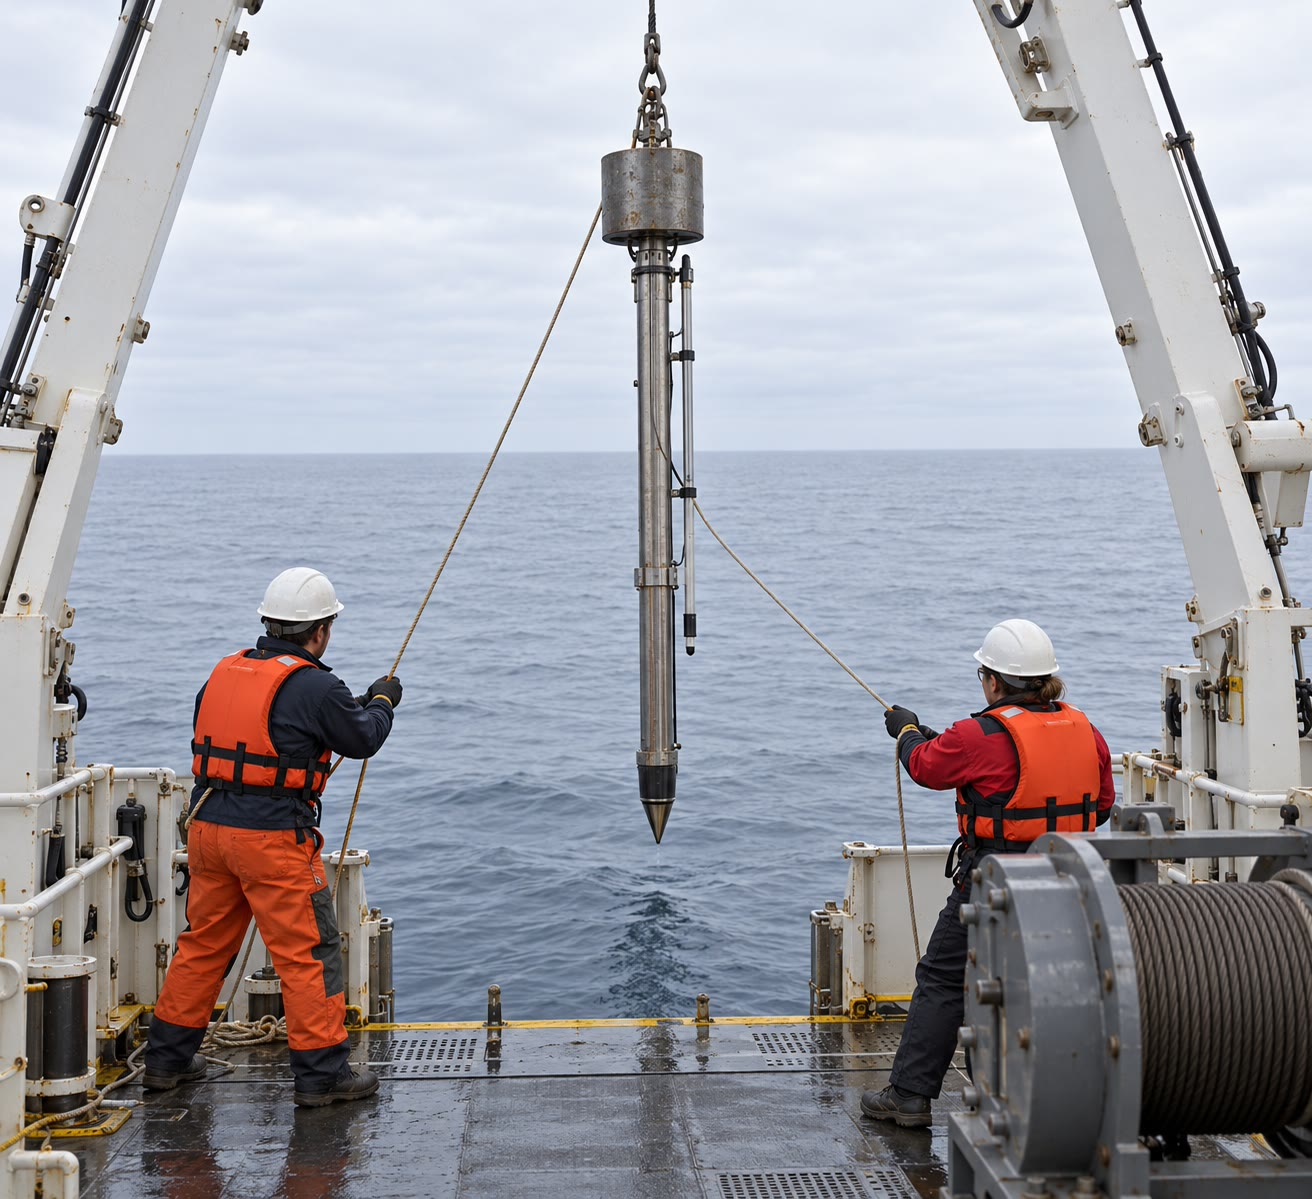
\includegraphics[width=\linewidth]{images/book5/ai/b3-heatflow-probe.jpg}

{\scriptsize Uma lança de fluxo de calor prestes a ser baixada da popa de um
navio de pesquisa. Ilustração gerada por IA.}
\end{minipage}
\end{inthefield}

\section*{Exercícios}

\begin{exercise}[$\star$]\label{exo:b3:lithosphere-thermal-models:1}
Com $\kappa = \qty{e-6}{m^2.s^{-1}}$, calcule o tempo condutivo $L^2/\kappa$
para $L = 1$, 10 e \qty{100}{km}, em milhões de anos.
\end{exercise}

\begin{exercise}[$\star$]\label{exo:b3:lithosphere-thermal-models:2}
Uma cadeia de montanhas é erodida a \qty{1}{mm/yr}, e a rocha sobe através da
\qty{30}{km} superiores da crosta para repô-la. Com $\kappa = \qty{e-6}{m^2.s^{-1}}$,
calcule o número de Péclet. A geoterma da cadeia pode ser calculada apenas por
condução?
\end{exercise}

\begin{exercise}[$\star$]\label{exo:b3:lithosphere-thermal-models:3}
No modelo de semiespaço ($T_0 = 0$, $T_m = \qty{1450}{\celsius}$, $\kappa =
\qty{0.8e-6}{m^2.s^{-1}}$), calcule a temperatura \qty{10}{km} abaixo do assoalho
oceânico com \qty{5}{Myr} de idade (\qty{1}{Myr} $= \qty{3.156e13}{s}$; $\operatorname{erf}
0.445 = 0.471$).
\end{exercise}

\begin{exercise}[$\star$]\label{exo:b3:lithosphere-thermal-models:4}
Com $C_q = \qty{490}{mW.m^{-2}.Myr^{1/2}}$, calcule o fluxo de calor através do
assoalho oceânico de 1, 25 e \qty{100}{Myr} de idade. Qual dos três seria o mais
provavelmente subestimado por uma sonda?
\end{exercise}

\begin{exercise}[$\star\star$]\label{exo:b3:lithosphere-thermal-models:5}
No modelo de semiespaço, a temperatura atinge \qty{90}{\percent} de $T_m$
onde $\operatorname{erf}\eta = 0.9$, $\eta = 1.163$. Com $\kappa =
\qty{0.8e-6}{m^2.s^{-1}}$, calcule essa profundidade para 10, 40 e \qty{100}{Myr}.
\end{exercise}

\begin{exercise}[$\star\star$]\label{exo:b3:lithosphere-thermal-models:6}
Com os valores do texto, o modelo de semiespaço fornece $C =
\qty{370.5}{m.Myr^{-1/2}}$. Mantendo todos os demais valores, qual coeficiente de expansão térmica
daria o valor ajustado de \qty{350}{m.Myr^{-1/2}}? Que outro parâmetro
poderia ser alterado em vez disso?
\end{exercise}

\begin{exercise}[$\star\star$]\label{exo:b3:lithosphere-thermal-models:7}
Calcule o fluxo de calor assintótico $kT_m/L$ do modelo de placa para $L =
\qty{95}{km}$, $T_m = \qty{1450}{\celsius}$, e para $L = \qty{125}{km}$,
$T_m = \qty{1350}{\celsius}$, com $k = \qty{3.1}{W.m^{-1}.K^{-1}}$ em ambos os casos.
Qual está mais próximo do fluxo de calor do assoalho oceânico antigo calculado a partir de $C_q/\sqrt t$
em \qty{150}{Myr} com $C_q = \qty{490}{mW.m^{-2}.Myr^{1/2}}$?
\end{exercise}

\begin{exercise}[$\star\star$]\label{exo:b3:lithosphere-thermal-models:8}
Uma província tem $q_0 = \qty{60}{mW.m^{-2}}$, $h_r = \qty{10}{km}$ e $A_0h_r =
0.4\,q_0$. Calcule $A_0$, $q_m$ e a temperatura no Moho, a \qty{35}{km}
de profundidade, com $k = \qty{2.5}{W.m^{-1}.K^{-1}}$.
\end{exercise}

\begin{exercise}[$\star\star$]\label{exo:b3:lithosphere-thermal-models:9}
Dois plútons graníticos de uma mesma província dão $q_0 = \qty{66}{mW.m^{-2}}$ com $A_0
= \qty{3.0}{\micro W.m^{-3}}$, e $q_0 = \qty{48}{mW.m^{-2}}$ com $A_0 =
\qty{1.2}{\micro W.m^{-3}}$. Supondo que eles estejam sobre a reta dada
pela \cref{prop:b3:lithosphere-thermal-models:exponential}, calcule $h_r$ e $q_m$.
\end{exercise}

\begin{exercise}[$\star\star\star$]\label{exo:b3:lithosphere-thermal-models:10}
(a) Mostre que o calor perdido através do assoalho oceânico entre as idades 0 e $t$, por
unidade de área, é $Q(t) = 2k(T_m - T_0)\sqrt{t/(\pi\kappa)}$ no modelo de
semiespaço. (b) Mostre que a subsidência é $d - d_r = \alpha Q/\bigl(c(\rho_m -
\rho_w)\bigr)$, em que $c = k/(\rho_m\kappa)$ é o calor específico. (c) Verifique-o
numericamente, para \qty{40}{Myr}, com os valores do texto.
\end{exercise}

\begin{exercise}[$\star\star\star$]\label{exo:b3:lithosphere-thermal-models:11}
No modelo de placa do texto ($\tau = \qty{36.2}{Myr}$, $\rho_m\alpha T_mL/
\bigl(2(\rho_m - \rho_w)\bigr) = \qty{3104}{m}$), a profundidade calculada com o
primeiro termo de Fourier isoladamente excede a série completa principalmente pelo termo $n = 3$.
Calcule o tamanho desse termo para 1, 10 e \qty{20}{Myr}, e a idade a partir da qual
o primeiro termo isolado fica a menos de \qty{10}{m} da série.
\end{exercise}

\begin{exercise}[$\star\star\star$]\label{exo:b3:lithosphere-thermal-models:12}
(a) Mostre que, na geoterma dada pela \cref{prop:b3:lithosphere-thermal-models:exponential},
$T(z) \approx q_mz/k + A_0h_r^2/k$ para $z \gg h_r$. (b) Deduza a profundidade da
isoterma de \qty{1300}{\celsius} para $q_0 = \qty{40}{mW.m^{-2}}$, com os valores
do exercício 8. (c) Quanto $q_m$ deve diminuir para que essa profundidade atinja
\qty{250}{km}, a profundidade das raízes rápidas dos crátons?
\end{exercise}

\section{Problema: quarenta milhões de anos afastado da dorsal}

\begin{problem}[{Problema de fim de semana --- o semiespaço e a placa, a profundidade de
um oceano inventado, e a espessura de sua placa}]
\label{pb:b3:lithosphere-thermal-models:1}
% values: calc/ch05.py; plate_cooling.py; honda04:gdh1, ps77:depth-age, data:b5-depth-age
Tome $T_0 = 0$, $T_m = \qty{1450}{\celsius}$, $\kappa =
\qty{0.8e-6}{m^2.s^{-1}}$, $k = \qty{3.1}{W.m^{-1}.K^{-1}}$, $\alpha =
\qty{3.1e-5}{K^{-1}}$, $\rho_m = \qty{3300}{kg.m^{-3}}$, $\rho_w =
\qty{1030}{kg.m^{-3}}$, uma dorsal com \qty{2500}{m} de profundidade, e \qty{1}{Myr} $=
\qty{3.156e13}{s}$.

\medskip\noindent\textbf{Parte I --- O semiespaço.}
\begin{enumerate}
  \item Calcule $\sqrt{\kappa t}$ para 10 e \qty{40}{Myr}.
  \item Calcule a temperatura \qty{20}{km} abaixo do assoalho nas duas idades
        ($\operatorname{erf}0.6294 = 0.6266$, $\operatorname{erf}0.3147 =
        0.3437$).
  \item A isoterma de \qty{1000}{\celsius} fica onde $\operatorname{erf}\eta =
        0.6897$, $\eta = 0.7174$. Calcule sua profundidade nas duas idades e a idade
        em que ela atinge \qty{60}{km}.
  \item Calcule o fluxo de calor nas duas idades, e $C_q$.
  \item Uma dorsal se abre a \qty{25}{mm/yr} para cada lado. Calcule o número de Péclet
        da placa sobre \qty{95}{km}. Por que cada coluna pode ser resfriada
        isoladamente?
  \item Calcule o tempo condutivo através de \qty{95}{km}. O que ele diz de
        um modelo de semiespaço para um assoalho com \qty{150}{Myr} de idade?
\end{enumerate}

\medskip\noindent\textbf{Parte II --- A subsidência.}
\begin{enumerate}[resume]
  \item Recorde o equilíbrio isostático que transforma o déficit de temperatura de
        uma coluna em subsidência, e por que a integral pode ser estendida até o
        infinito no semiespaço.
  \item Calcule $C$ da lei profundidade--idade, e as profundidades em 10 e
        \qty{40}{Myr}.
  \item A profundidade mediana do assoalho oceânico real entre 40 e \qty{45}{Myr}
        é \qty{4475}{m}, sem correção. Compare com o modelo em
        \qty{42.5}{Myr}, e liste o que a mediana inclui e que o modelo
        deixa de fora.
  \item De quanto mudaria $C$ se $T_m$ fosse \qty{1350}{\celsius}?
        Compare com o valor ajustado de \qty{350}{m.Myr^{-1/2}}.
  \item Por que os fluxos de calor medidos em assoalho jovem ficam abaixo de $C_q/\sqrt t$?
\end{enumerate}

\medskip\noindent\textbf{Parte III --- A placa.} Tome $L = \qty{95}{km}$.
\begin{enumerate}[resume]
  \item Calcule $\tau$ e a amplitude $\rho_m\alpha T_mL/\bigl(2(\rho_m -
        \rho_w)\bigr)$.
  \item Calcule a profundidade em \qty{40}{Myr} com os termos $n = 1$, 3 e 5.
  \item Quanto o primeiro termo sozinho difere desse valor, e por que tão
        pouco?
  \item Calcule a diferença entre o semiespaço e a placa em 40 e
        \qty{50}{Myr}, e estime por interpolação linear a idade em que
        ela atinge \qty{100}{m}.
  \item Calcule o fluxo de calor da placa em \qty{40}{Myr}, com os termos
        $n = 1$ a 3, e compare com o semiespaço.
  \item Dê a profundidade e o fluxo de calor assintóticos.
\end{enumerate}

\medskip\noindent\textbf{Parte IV --- Um oceano inventado.} Em um oceano inventado
cuja dorsal está a \qty{2500}{m} de profundidade, o assoalho, uma vez corrigido
de sedimentos e afastado de montes submarinos e elevações, está a \qty{5700}{m}
de profundidade em \qty{120}{Myr} e a \qty{4800}{m} em \qty{40}{Myr}. O $L$ da
placa é desconhecido; todos os outros valores são os acima.
\begin{enumerate}[resume]
  \item Mantendo apenas o primeiro termo de Fourier, escreva a profundidade em
        \qty{120}{Myr} como função de $L$, com $\tau$ dependendo ele próprio de
        $L$.
  \item Resolva para $L$ por iteração, partindo de $L = \qty{100}{km}$:
        calcule $\tau$, depois o $L$ que corresponde a \qty{5700}{m} com esse
        $\tau$, e repita.
  \item Com o $L$ encontrado, calcule a profundidade em \qty{40}{Myr} e compare
        com o semiespaço e com os \qty{4800}{m} medidos.
  \item Calcule $\tau$ para esse $L$ e a profundidade assintótica deste oceano.
  \item Após que idade o assoalho está a menos de \qty{100}{m} de sua
        profundidade assintótica?
  \item Dê a espessura $L$ da placa que se ajusta ao assoalho antigo do
        oceano inventado.
\end{enumerate}
\end{problem}
